\section{Die Brownsche Bewegung}

Oft wird die Brownsche Bewegung (oder auch Wiener Prozess) axiomatisch definiert. In dieser Arbeit werden 
direkt kumulative Normalverteilungen betrachtet. Zuerst wird eine vereinfachte Darstellung des Prozesses eingeführt, 
die diskrete Brownsche Bewegung.

\subsection{Diskrete Brownsche Bewegung}

\begin{defi}[Diskrete Brownsche Bewegung]
Die elementare Brownsche Bewegung sei ein stochastischer Prozess, 
der aus einer Folge von Zufallsvariablen $\xi_n, n \in \Bbb N_0$ besteht, wobei
$$\xi_n = \sum_{i=1}^n \eta_i, \quad \eta_i \sim N(0,1)$$. 
Die Zufallsvariablen $\eta_i$ sind unabhängig und identisch verteilt. Nun 
Nun wird eine stetige Zeitentwicklung durch lineare Interpolation eingeführt:
$$b^{(1)}(t) := \xi_{\lfloor t \rfloor} + (t - \lfloor t \rfloor)(\xi_{\lfloor t \rfloor + 1} - \xi_{\lfloor t \rfloor}), \quad t \geq 0.$$
Die Funktion $b{(1)}(t)$ wird diskrete Brownsche Bewegung erster Ordnung genannt.
Der Name rührt daher, dass in eine Zeiteinheit genau eine Normalverteilung einbezogen wird.
Im Allgemeinen wird die diskrete Brownsche Bewegung $b^{(N)}(t)$ $N$-ter Ordnung definiert als
$$b^{(N)}(t) := \frac{1}{\sqrt{N}} \left ( \xi_{\lfloor Nt \rfloor} + (Nt - \lfloor Nt \rfloor)(\xi_{\lfloor Nt \rfloor + 1} - \xi_{\lfloor Nt \rfloor}) \right ), \quad t \geq 0.$$
Hierbei wird in eine Zeiteinheit $N$ Normalverteilungen einbezogen.

\end{defi}

\begin{bsp}[Visualisierung der diskreten Brownschen Bewegung]
Das folgende R-Programm (Ausschnitt) generiert eine diskrete Brownsche Bewegung N-ter Ordnung:

\begin{lstlisting}
  n_points <- N * T_max
  eta <- rnorm(n_points, mean=0, sd=1)
  xi <- c(0, cumsum(eta))
  t_grid <- seq(0, T_max, length.out=steps)
  k <- floor(N * t_grid)
  frac <- N * t_grid - k
  vals <- xi[k+1] + frac * (xi[k+2] - xi[k+1])
  vals <- vals / sqrt(N)
\end{lstlisting}
Für verschiedene Werte von $N$ ergeben sich die folgenden Grafiken:

\begin{figure}[H]
    \centering
    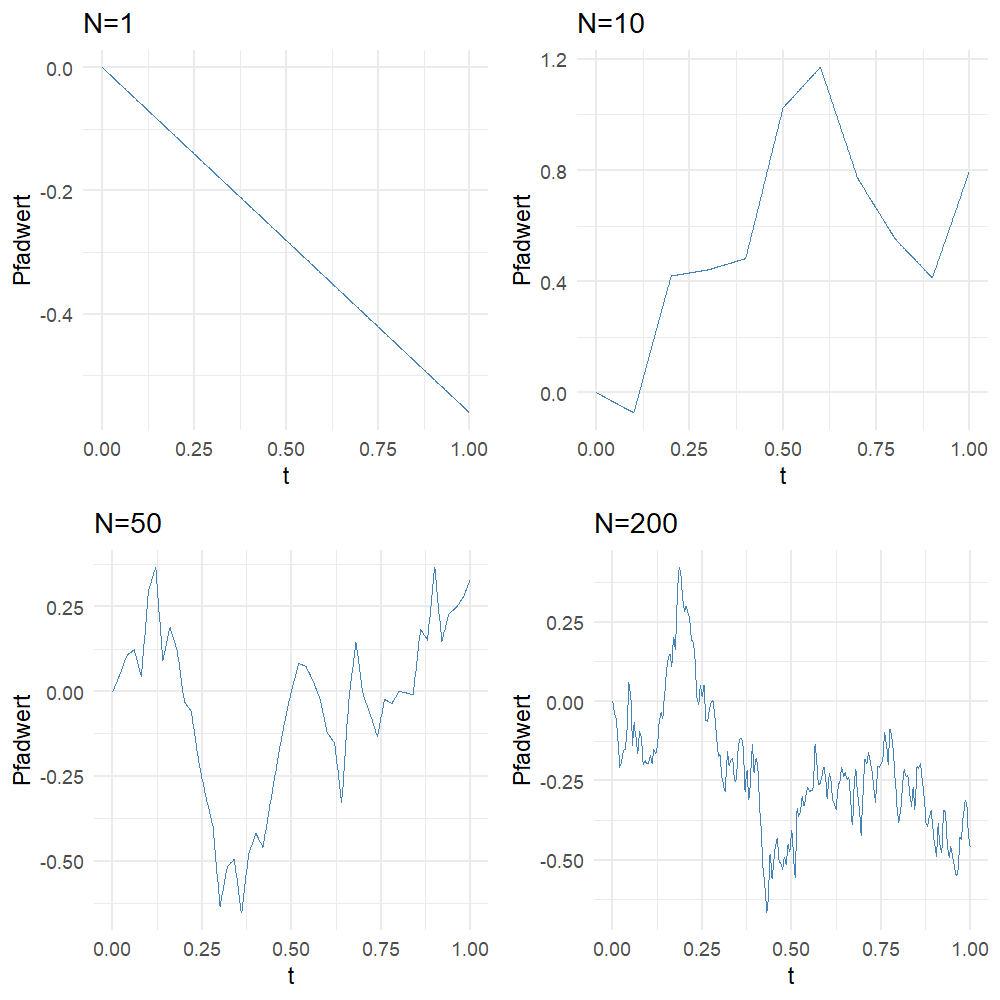
\includegraphics[width=0.9\textwidth]{images/disrete_bb.png}
    \caption{Diskrete Brownsche Bewegung erster, zehnter, fünfzigster und zweihundertster Ordnung}
    \label{fig:brownian}
\end{figure}

\end{bsp}

\begin{lemma}[Martingal-Eigenschaft der diskreten Brownschen Bewegung]
Ohne Beschränkung der Allgemeinheit wird der Fall $N=1$ betrachtet, sonst kann die Zeit skaliert werden.
Ebenso wird nur der Fall $t \in \Bbb N_0$ untersucht: Der Prozess ist also wieder diskret. Das ist
ausreichend, da im Verlauf der Arbeit der Grenzprozess $N \to \infty$ relevant 
wird. Dann ist jeder Wert der Brownschen Bewegung beliebig nah an einem der diskreten Werte, 
und die Martingal-Eigenschaft folgt aus der Stetigkeit des Erwartungswertes. Der stetig interpolierte 
diskrete Prozess an sich ist nämlich kein Martingal. \textit{Beweis.}
Zuerst wird der Fall $m=n+1$ betrachtet: zu zeigen ist
$$E(b^{(1)}(m) | b^{(1)}(n)=v) = v.$$
Da $b^{(1)}(m) = b^{(1)}(n) + \eta_{n+1}$ folgt
$$E(b^{(1)}(m) | b^{(1)}(n)=v) = E(v + \eta_{n+1} | b^{(1)}(n)=v) = v + E(\eta_{n+1}) = v.$$
Nun der allgemeine Fall $m > n+1$: aus dem Satz des iterierten Erwartungswertes folgt
$$E(b^{(1)}(m) | b^{(1)}(n)=v) = E(E(b^{(1)}(m) | b^{(1)}(m-1)) | b^{(1)}(n)=v).$$
Da $E(b^{(1)}(m) | b^{(1)}(m-1)) = b^{(1)}(m-1)$ folgt
$$E(b^{(1)}(m) | b^{(1)}(n)=v) = E(b^{(1)}(m-1) | b^{(1)}(n)=v).$$
Induktiv folgt die Behauptung. \qed \\

\end{lemma}

\begin{lemma}[Varianz der diskreten Brownschen Bewegung]
$$
\begin{aligned}
V(b^{(N)}(t)) &= \frac{1}{N} \left ( V(\xi_{\lfloor Nt \rfloor}) + (Nt - \lfloor Nt \rfloor)^2 \text{Var}(\xi_{\lfloor Nt \rfloor + 1} - \xi_{\lfloor Nt \rfloor}) \right ) 
\\ &= \frac{1}{N} (\lfloor Nt \rfloor + (Nt - \lfloor Nt \rfloor)^2)  
\\ &= \frac{\lfloor Nt \rfloor}{N} + \frac{(Nt - \lfloor Nt \rfloor)^2}{N}.
\end{aligned}
$$
Im Grenzübergang $N \to \infty$ konvergiert $\frac{\lfloor Nt \rfloor}{N} \to t$ und $\frac{(Nt - \lfloor Nt \rfloor)^2}{N} \to 0$.
\end{lemma}

\subsection{Ausgewählte Ergebnisse aus der Stochastik}
Im Folgenden Beweis zur Stetigkeit der Pfade werden einige Ergebnisse aus der Stochastik verwendet, die hier zusammengefasst, aber nicht bewiesen werden.

\begin{lemma}[Reihenkriterium für fast sichere Konvergenz, \cite{henze} S. 201]
Sei $(X_n)_{n \in \Bbb N}$ eine Folge von Zufallsvariablen. Wenn es eine Reihe $\sum_{n=1}^\infty a_n \lt \infty$ mit $a_n \geq 0$ gibt, so dass
$$P(|X_n| > \varepsilon) \leq a_n \quad \text{für alle } n \in \Bbb N \text{ und jedes } \varepsilon > 0,$$
dann konvergiert $X_n$ fast sicher gegen $0$, d.h.
$$P\left(\lim_{n \to \infty} X_n = 0\right) = 1.$$
\end{lemma}

\begin{lemma}[Kolmogorov-Ungleichung, \cite{henze} S. 207]
Seien $X_1, X_2, \ldots, X_n$ unabhängige Zufallsvariablen mit $E(X_i) = 0$ und $V(X_i) < \infty$ für alle $i=1, \ldots, n$. Dann gilt für jedes $\varepsilon > 0$
$$P\left(\max_{1 \leq k \leq n} |S_k| \geq \varepsilon \right) \leq \frac{1}{\varepsilon^2} V(S_n),$$
wobei $S_k := \sum_{i=1}^k X_i$.
\end{lemma}

\subsection{Die Brownschen Bewegung als Grenzprozess}
Nun wird der Grenzprozess $N \to \infty$ betrachtet. Intuitiv wird die Zeit immer feiner aufgelöst,
und es werden immer mehr Normalverteilungen in eine Zeiteinheit einbezogen. Vorerst ist jedoch unklar, 
ob der Grenzprozess überhaupt existiert.

\begin{satz}[Existenz der Brownschen Bewegung]
Es existiert ein stochastischer Prozess $W_t, t \geq 0$, so dass für jedes $t$ die Verteilung von $b^{(N)}(t)$ gegen die Verteilung von $W_t$ konvergiert, wenn $N \to \infty$.
\textit{Beweis.}
Da 
$$b^{(N)}(t) = \frac{1}{\sqrt{N}}\big(\xi_k+\alpha(\xi_{k+1}-\xi_k)\big)
=\frac{1}{\sqrt{N}}\big(\xi_k+\alpha\,\eta_{k+1}\big).
$$
ist $b^{(N)}(t)$ eine lineare Kombination von Normalverteilungen, und daher widerum 
normalverteilt. Erwartungswert und Varianz wurden bereits berechnet:
$$
E(b^{(N)}(t)) = 0, \quad V(b^{(N)}(t)) = \sigma_N^2(t) = \frac{1}{N}\big(k+\alpha^2\big),
$$
wobei $k=\lfloor Nt \rfloor$ und $\alpha=Nt-k\in[0,1)$. Damit gilt
$$
b^{(N)}(t) \sim N\left(0,\frac{1}{N}\big(k+\alpha^2\big)\right).
$$
Die Verteilungsfunktion ist gegeben durch
$$
F_N(x)=\Bbb P\big(b^{(N)}(t)\le x\big)=\Phi\!\left(\frac{x}{\sigma_N(t)}\right),
$$
wobei $\Phi$ die Standardnormalverteilungsfunktion ist. Aus $\sigma_N^2(t)\to t$ folgt $\sigma_N(t)\to \sqrt{t}$ und wegen der Stetigkeit von $\Phi$ daher
$$
F_N(x)=\Phi\!\left(\frac{x}{\sigma_N(t)}\right)\;\longrightarrow\;\Phi\!\left(\frac{x}{\sqrt{t}}\right)\quad\text{für alle }x\in\Bbb R.
$$
Dies ist die Verteilungsfunktion von $N(0,t)$. Definiere $W_t\sim N(0,t)$. Somit konvergiert für jedes feste $t$ die Verteilung von $b^{(N)}(t)$ gegen die von $W_t$. 
\qed
\end{satz}

\begin{satz}[Stetigkeit der Pfade]
Der Pfad $t \mapsto W_t(\omega)$ ist fast sicher stetig.
\textit{Beweis.}
Für den Beweis wird eine neue Funktionen-Folge $\hat W_t^{(n)}(\omega), n \in \Bbb N$
definiert, wobei $\hat W_t^{(n)}(\omega)$ die lineare Interpolation der Werte $W_{k/2^n}(\omega), k=0,1,2,\ldots$ ist. 
Ohne Beschränkung der Allgemeinheit wird das Intervall $[0,1]$ betrachtet. Für $n \in \Bbb N$ und $k=0,\dots,2^n-1$ setze
$$I_{n,k}:=\big[k2^{-n},(k+1)2^{-n}\big].$$
Da die $I_{n,k}$ eine Zerlegung von $[0,1]$ bilden, ist
$$
\begin{aligned}
M_n &:=\sup_{t\in[0,1]}\big|\hat W^{(n+1)}_t-\hat W^{(n)}_t\big| 
\\ &= \max_{0\le k<2^n} \sup_{t\in I_{n,k}} \big|\hat W^{(n+1)}_t-\hat W^{(n)}_t\big| =\max_{0\le k<2^n}|Z_{n,k}|
\end{aligned}
$$
Für die unabhängigen Inkremente $Z_{n,k}$ mit
$$Z_{n,k}\sim N\!\big(0,2^{-(n+2)}\big).$$
Mit der Kolmogorov-Ungleichung erhält man für jedes $\varepsilon>0$
$$
\Bbb P(M_n>\varepsilon) \le \frac{1}{\varepsilon^2} V(Z_{n,0}) = \frac{1}{\varepsilon^2} 2^{-(n+2)}.
$$
Wähle nun $\varepsilon_n:=2^{-n/4}$. Dann gilt
$$
\sum_{n=1}^\infty \Bbb P\!\big(M_n>\varepsilon_n\big)
\le \sum_{n=1}^\infty 2^{n/2} \cdot 2^{-(n+2)}<\infty.
$$
Nach dem Reihenkriterium für fast sichere Konvergenz folgt, dass $M_n\to 0$ fast sicher.
Für $m \gt n \ge N$ beliebig gilt
$$\sup_{t}|\hat W^{(m)}_t - \hat W^{(n)}_t| \leq \sum_{k=n}^{m-1} M_k. \underset{N \to \infty} \longrightarrow 0$$
Weil jedes $\big(\hat W^{(n)}\big)_{n\in\Bbb N}$ eine stückweise lineare Funktion ist, folgt
dass $\big(\hat W^{(n)}\big)_{n\in\Bbb N}$ fast sicher eine Cauchy-Folge in $\Vert \cdot \Vert_{\infty}$ ist.
$\big(\hat W^{(n)}\big)_{n\in\Bbb N}$ konvergiert also gleichmäßig gegen den Grenzpfad $\widetilde W$, der stetig ist. \qed

Achtung: Es wurde nicht gezeigt, der Prozess $W_t^{(n)} \longrightarrow W_t$ gleichmäßig konvergiert. Für eine feste Realisierungen
$t \mapsto W_t(\omega)$ wurde eine (reellwertige) Folge von stetigen Funktionen konstruiert, die gegen eine stetige Funktion gleich konvergiert.
\end{satz}

\subsection{Eigenschaften der Brownschen Bewegung}

\begin{satz}[Selbstähnlichkeit der Brownschen Bewegung]
Für jedes $c > 0$ gilt
$$
\begin{aligned}
W_{ct}(\omega) &\stackrel{d}{=} \sqrt{c} W_t(\omega) \quad \text{für alle } t \ge 0.
\end{aligned}
$$
und für alle $s \lt t$ gilt
$$
W_t - W_s \sim N(0, t-s).
$$
\textit{Beweis der ersten Behauptung.}
Für $t \ge 0$ sei $k = \lfloor Nt \rfloor$ und $\alpha = Nt - k \in [0,1)$. Dann gilt
$$
W_{ct}(\omega) = \lim_{N \to \infty} b^{(N)}_{ct}(\omega) = \lim_{N \to \infty} \frac{1}{\sqrt{N}} \left( \xi_k + \alpha (\xi_{k+1} - \xi_k) \right) = \sqrt{c} W_t(\omega).
$$
\textit{Beweis der zweiten Behauptung.}
Für $s < t$ gilt
$$
W_t - W_s = \lim_{N \to \infty} \left( b^{(N)}(t) - b^{(N)}(s) \right).
$$
Da $b^{(N)}(t) - b^{(N)}(s)$ eine Normalverteilung mit Erwartungswert $0$ und Varianz $t-s$ hat, folgt aus der Verteilungskonvergenz, dass
$$
W_t - W_s \sim N(0, t-s).
$$
\qed

\end{satz}

\begin{satz}[Varianz der Brownschen Bewegung]
Die Brownsche Bewegung $W_t$ hat die Varianz $V(W_t) = t$.
\textit{Beweis.}
Aus der gleichmäßigen Konvergenz von $b^{(N)}(t)$ gegen $W_t$ folgt, dass die Verteilung von $b^{(N)}(t)$ für jedes $t$ gegen die Verteilung von $W_t$ konvergiert. Da die Varianz eine Eigenschaft der Verteilung ist, gilt
$$
V(W_t) = \lim_{N \to \infty} V(b^{(N)}(t)) = t.
$$
\qed
\end{satz}

\begin{satz}[Martingal-Eigenschaft der Brownschen Bewegung]
Die Brownsche Bewegung $W_t$ ist ein Martingal.
\textit{Beweis.}
Die diskrete Brownsche Bewegung $b^{(N)}(t)$ ist ein Martingal, wie bereits gezeigt wurde.
Außerdem ist die Verteilungskonvergenz von $b^{(N)}(t)$ gegen $W_t$ ist gegeben.
Verteilungskonvergenz impliziert Konvergenz des Erwartungswertes (Henze), also
$$
E(W_t) = \lim_{N \to \infty} E(b^{(N)}(t)) = 0.
$$
Aus der Selbstähnlichkeit der Brownschen Bewegung $$W_t - W_s \sim N(0, t-s)$$
folgt, dass $W_t - W_s$ unabhängig von $W_s$ ist. Somit gilt
$$
E(W_t | W_s = v) = E(W_t - W_s + v | W_s = v) = E(W_t - W_s) + v = v.
$$

Damit ist $W_t$ ein Martingal. \qed
\end{satz}